\documentclass[conference]{IEEEtran}
\usepackage{graphicx}
\usepackage{booktabs}
\usepackage{array}
\usepackage{amsmath}
\usepackage{url}
\usepackage[hidelinks]{hyperref}
\usepackage{cite}

\begin{document}

\title{Load-Aware UPF Scaling and Performance Evaluation in a 5G Core}

\author{
\IEEEauthorblockN{Suthar Jainish Chandraprakash \quad Gomtesh}
\IEEEauthorblockA{Indian Institute of Technology Gandhinagar\\
5G and Beyond Projects 2026\\
suthar.jainish@iitgn.ac.in, gomtesh@iitgn.ac.in}
}

\maketitle

\begin{abstract}
We study when a single User Plane Function (UPF) in a 5G core starts to degrade and whether a second UPF, started on demand, helps. We build a testbed from Open5GS, UERANSIM and iperf3 in Docker Compose, cap each UPF at 0.1 CPU core so it saturates before the traffic generator does, and measure throughput, loss, round-trip time and UPF CPU as load rises. One UPF carries about 68~Mbit/s and degrades from about 60~Mbit/s. A small controller that watches UPF CPU starts a second UPF at 80\% of the cap. With 96~Mbit/s offered, this cuts loss from 27.9\% to 3.9\%, while starting with two UPFs gives 0.0\%. Traces of the N4 and N3 interfaces show that Open5GS places new sessions strictly in round-robin order and never moves existing ones, which explains the remaining gap. We also show how to retire the second UPF without losing traffic, and list the configuration needed and the limits we found.
\end{abstract}

\begin{IEEEkeywords}
5G core, UPF, Open5GS, UERANSIM, scaling, PFCP, GTP-U
\end{IEEEkeywords}

\section{Introduction}
The UPF carries all user traffic in a 5G network. When one UPF runs out of CPU, packets are delayed and dropped, so operators add UPF instances. The 3GPP architecture lets the Session Management Function (SMF) control several UPFs over the N4 (PFCP) interface~\cite{ts23501,ts29244}, but it does not say when to add one or how new sessions are spread over them.

This project answers four practical questions on an open-source core. (1) At what load does one UPF degrade? (2) Can a second UPF join while the core is running, without restarting it? (3) Can a simple controller decide when to add and remove it? (4) How much does the second UPF help, and what stops it from helping more? All numbers come from one test bed and one measurement session, described in Section~\ref{sec:setup}.

\section{Test Bed}\label{sec:setup}
Fig.~\ref{fig:arch} shows the setup. The core is Open5GS 2.8.0 (AMF, SMF, NRF, UDM, UDR, AUSF, PCF, NSSF in one container, subscribers in MongoDB)~\cite{open5gs}. The gNB and the simulated UEs run in UERANSIM 3.2.6~\cite{ueransim}. The data network is one container running 60 iperf3 servers, one per UE. Each UPF is its own container with separate N3 (gNB side), N4 (SMF side) and N6 (data network side) addresses. Everything is started with Docker Compose.

\begin{figure}[t]
\centering
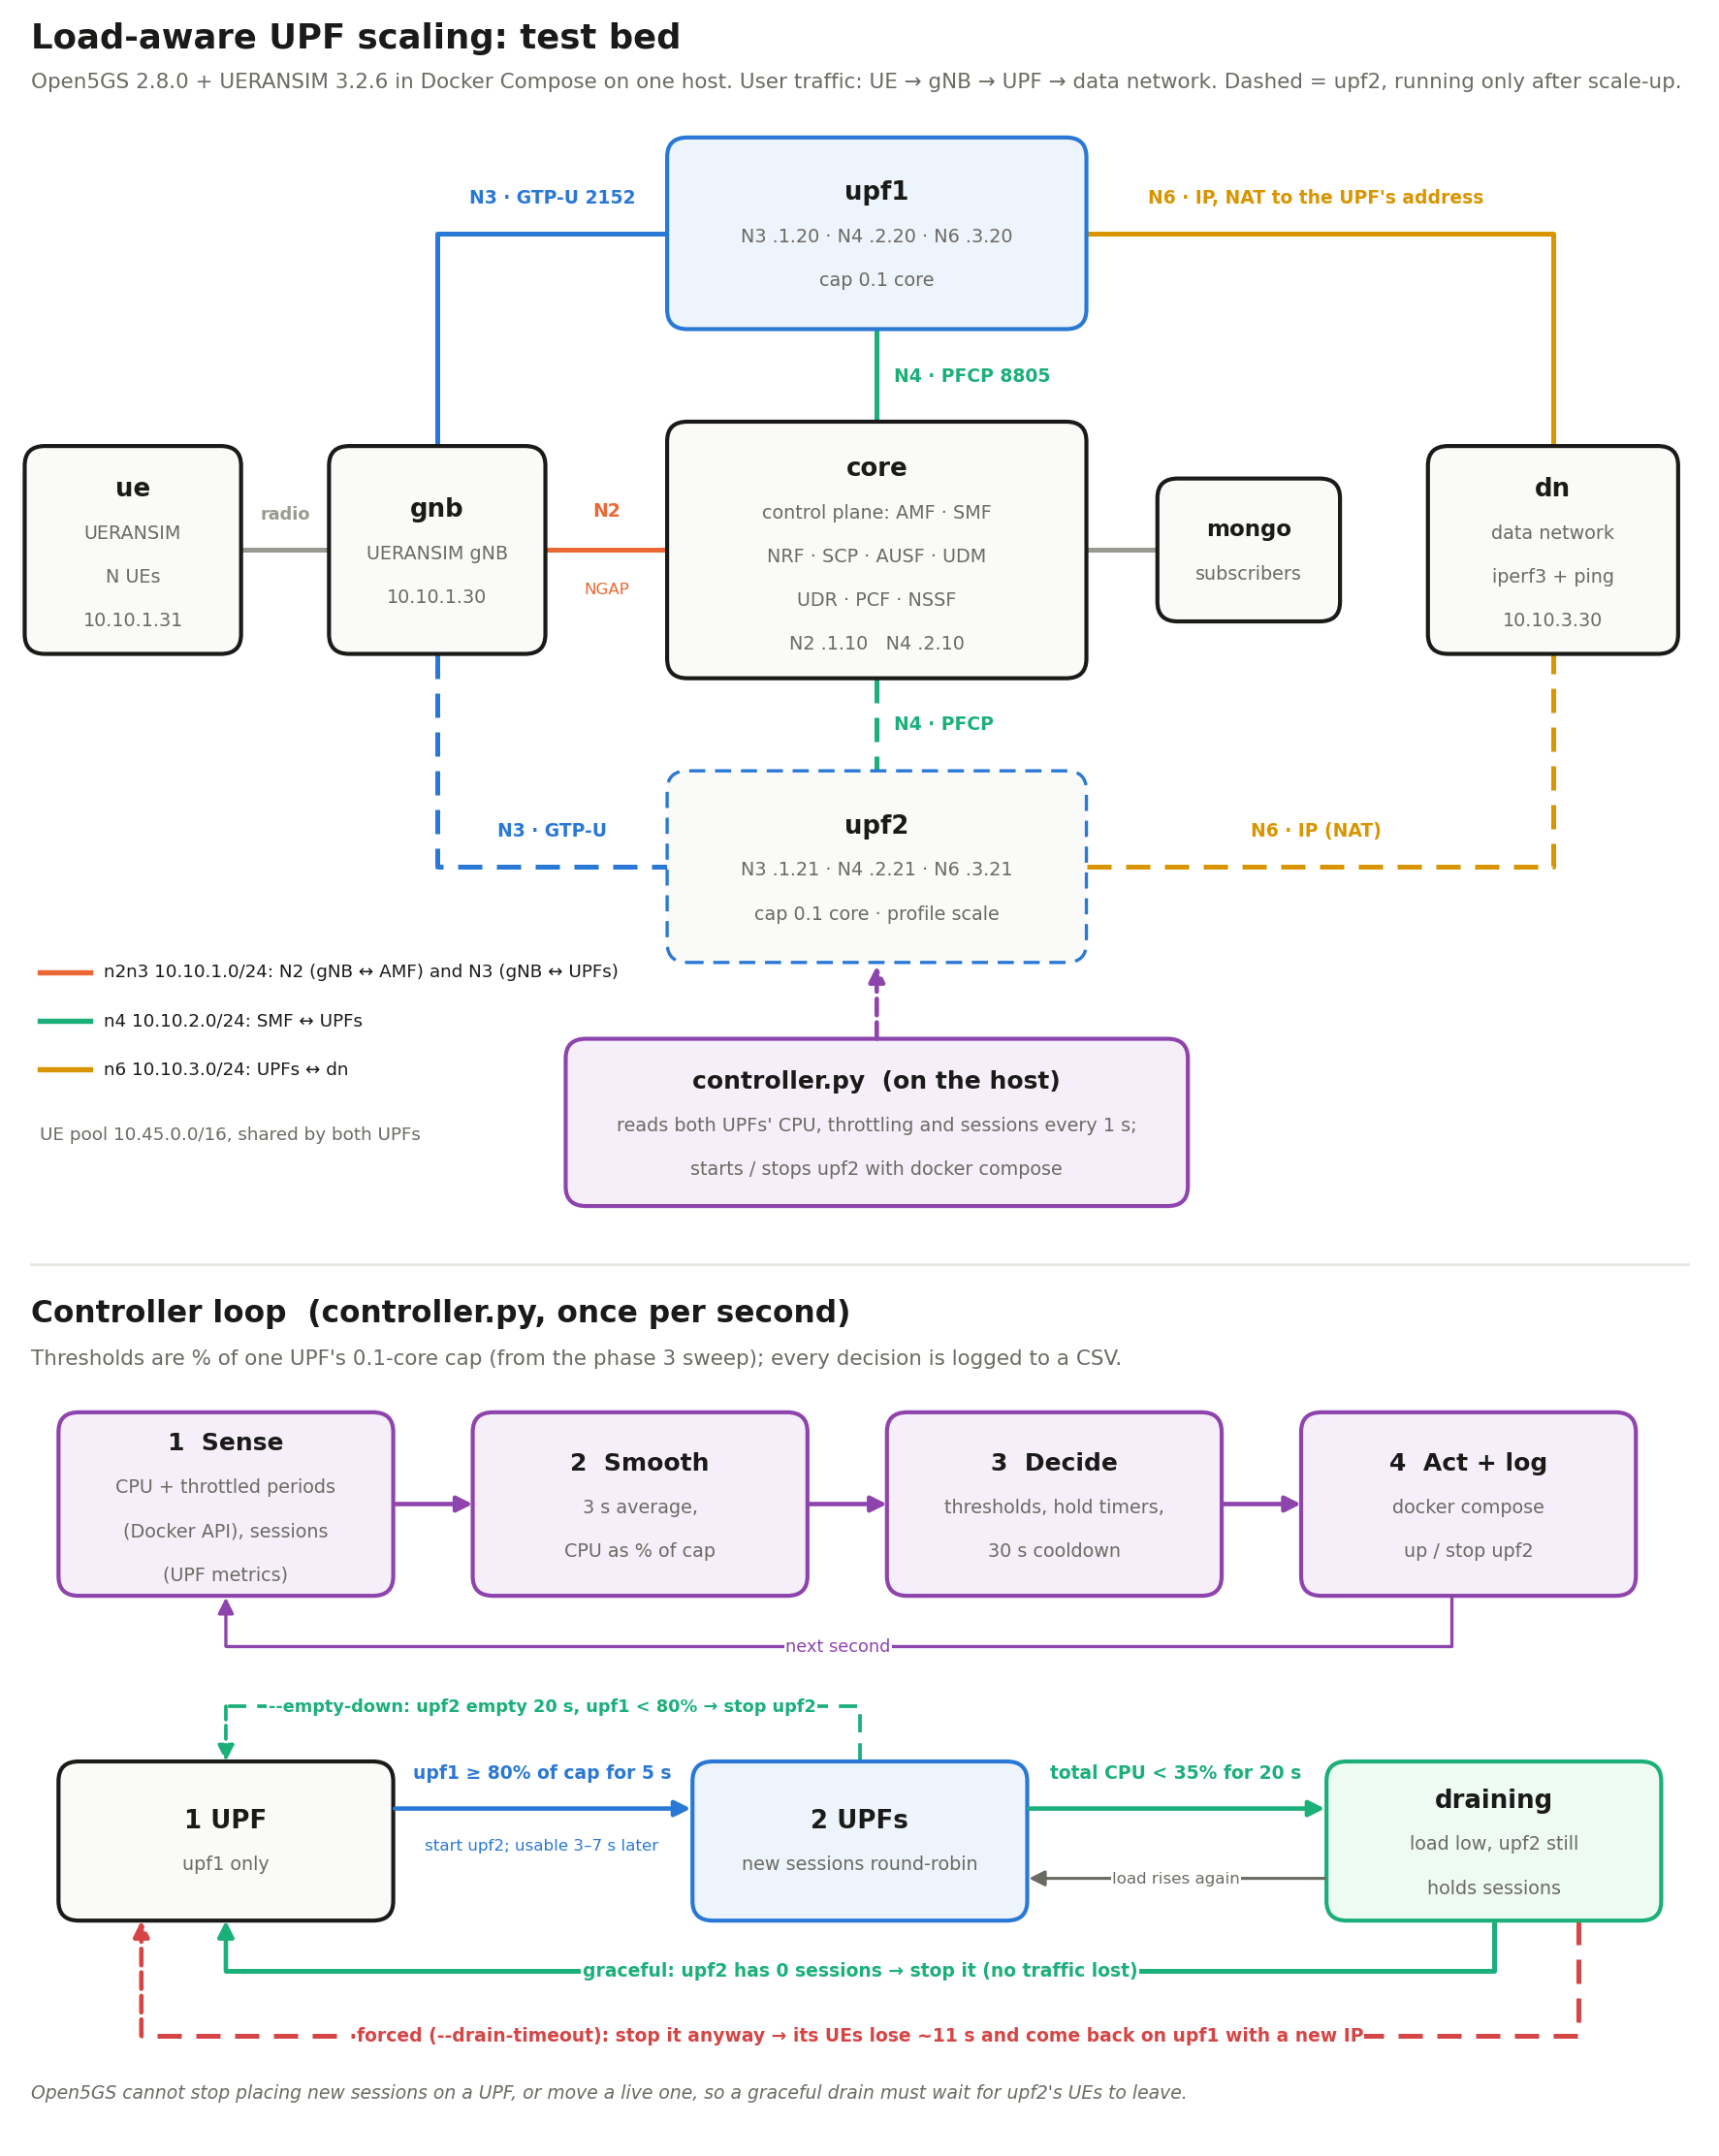
\includegraphics[width=\columnwidth]{architecture.png}
\caption{Test bed and controller loop. The controller reads UPF CPU through the Docker API and starts or stops the second UPF.}
\label{fig:arch}
\end{figure}

\textbf{CPU cap.} UERANSIM cannot generate enough traffic to saturate an uncapped UPF. We therefore limit each UPF to 0.1 core (1~ms of CPU per 10~ms period). The cap is artificial, so absolute Mbit/s figures are not real UPF capacities; the shape of the results is what matters.

\textbf{Measurements.} Each run sends uplink UDP from several UEs through the UPF to the data network. We record delivered throughput, loss (from iperf3), RTT (ping through one tunnel), UPF CPU as a share of its cap, the share of 10~ms periods in which the UPF was throttled, and the number of sessions. CPU and throttling are read through the Docker Engine API, never with \texttt{docker exec} inside the UPF, because an early version of the tool did exactly that and added about 4\% CPU and 50\% throttling at idle. Failed steps are retried and flagged, and the order of loads is shuffled.

\textbf{Host.} The final results were measured in one session on a 12-core Linux laptop on AC power, CPU governor \texttt{performance}, nothing else running (host load 0.3 at the start; the 1-minute load average peaked at 3.2 during the sweep and stayed below 2.3 in the ramp runs). Earlier runs on a laptop with Docker Desktop were used for development only and are not used for the figures below.

\section{Where One UPF Degrades}\label{sec:threshold}
We offered 10--120~Mbit/s from 4 UEs, four shuffled repetitions per load. All 40 runs were valid (no failed iperf3, no dead tunnels). Table~\ref{tab:thr} gives the medians.

\begin{table}[t]
\centering
\caption{One UPF at 0.1 core: medians over four runs.}
\label{tab:thr}
\footnotesize
\setlength{\tabcolsep}{2.2pt}
\begin{tabular}{lrrrrrrrrr}
\toprule
Offered (Mbit/s) & 20 & 30 & 40 & 50 & 60 & 70 & 80 & 100 & 120 \\
\midrule
Delivered (Mbit/s) & 20.0 & 30.0 & 39.8 & 49.7 & 59.4 & 66.4 & 67.7 & 66.5 & 63.2 \\
Loss (\%) & 0.0 & 0.01 & 0.4 & 0.7 & 1.0 & 5.1 & 15.4 & 33.5 & 47.3 \\
UPF CPU (\% of cap) & 42 & 58 & 71 & 87 & 95 & 98 & 98 & 98 & 98 \\
Throttled (\%) & 0.9 & 1.7 & 1.5 & 7.6 & 66.7 & 99.7 & 99.7 & 99.6 & 99.6 \\
RTT p95 (ms) & 0.31 & 0.30 & 0.29 & 0.29 & 3.7 & 10.4 & 13.3 & 15.4 & 16.5 \\
\bottomrule
\end{tabular}
\end{table}

\begin{figure}[t]
\centering
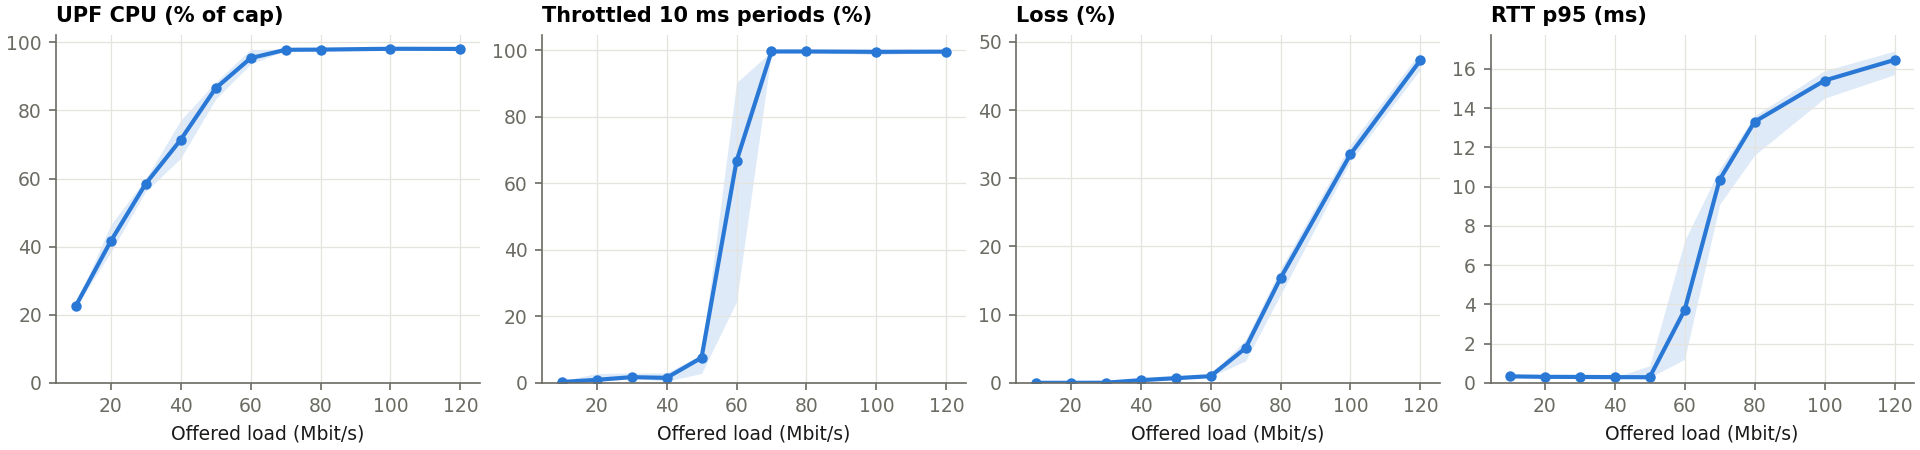
\includegraphics[width=\columnwidth]{threshold.png}
\caption{Load sweep for one UPF at 0.1 core.}
\label{fig:thr}
\end{figure}

Delivered throughput flattens at about 68~Mbit/s, and extra load only adds loss (47\% at 120 offered). The knee is at about 60~Mbit/s: throttling jumps to 67\% of periods and the RTT tail rises from 0.3 to 3.7~ms. Loss alone is a weak early signal (1\% at 60~Mbit/s), while CPU and throttling rise steadily and are the better signals.

\textbf{Scaling threshold.} A scale-up takes 5~s of holding time plus 3--7~s for the new UPF to associate, and it helps only sessions created afterwards. The trigger must therefore sit well below the knee. We use \textbf{UPF CPU $\geq$ 80\% of its cap} (or $\geq$ 50\% of periods throttled while CPU $\geq$ 75\%), held for 5~s, measured with a 3~s moving average. In this sweep that is about 46~Mbit/s (interpolated between the 40 and 50~Mbit/s points), roughly three quarters of the knee and two thirds of the capacity. A load of 30~Mbit/s (58\% CPU) never triggers it.

\textbf{Thresholds as percentages.} The cap is CPU time, so how many Mbit/s fit in it depends on the host. An earlier calibration on the same laptop with a slower CPU setting gave a capacity of 46~Mbit/s instead of 68, yet the same percentage thresholds again landed at about three quarters of the knee. We therefore express thresholds as a share of the cap and take all reported numbers from one session.

\section{Adding a Second UPF}\label{sec:second}
\subsection{Configuration}
The SMF is started with both UPF addresses in its list; only the first UPF runs at the start. The SMF keeps retrying the PFCP association with the absent one (about every 11~s) and uses it as soon as it answers, so no restart is needed. Table~\ref{tab:cfg} lists what must be set.

\begin{table}[t]
\centering
\caption{Open5GS settings needed for two UPFs.}
\label{tab:cfg}
\footnotesize
\setlength{\tabcolsep}{3pt}
\begin{tabular}{>{\raggedright\arraybackslash}p{3.3cm}>{\raggedright\arraybackslash}p{4.6cm}}
\toprule
Parameter & Purpose \\
\midrule
\texttt{smf.\allowbreak pfcp.\allowbreak client.\allowbreak upf[].\allowbreak address} & Every UPF the SMF may use must be listed (here 10.10.2.20 and .21). \\
\texttt{smf.\allowbreak pfcp.\allowbreak server.\allowbreak address} & Address the UPFs associate and send heartbeats to. \\
\texttt{smf.\allowbreak session[].\allowbreak subnet} & One UE address pool is shared by both UPFs; it cannot be tied to one UPF. \\
\texttt{upf[].\allowbreak dnn / tac / nr\_cell\_id} (SMF, optional) & Static selectors. Not set here, so the SMF alternates between UPFs. \\
\texttt{upf.\allowbreak pfcp.\allowbreak server.\allowbreak address} & Must equal the address in the SMF list. \\
\texttt{upf.\allowbreak gtpu.\allowbreak server.\allowbreak address} & N3 address sent to the gNB; uplink is tunnelled to it. \\
\texttt{upf.\allowbreak session[].\allowbreak subnet} & Each UPF must route the whole UE pool into its TUN device. \\
NAT on N6 (\texttt{iptables MASQUERADE}) & Both UPFs serve one pool, so the data network cannot tell which UPF owns an address. NAT sends replies back to the sending UPF. \\
Compose: own N3/N4/N6 IPs & Separate interfaces per UPF; a profile keeps upf2 off until needed. \\
\bottomrule
\end{tabular}
\end{table}

The AMF and gNB need no UPF-specific settings: the gNB learns each session's N3 address from the core.

\subsection{Session distribution}
We captured PFCP on N4 and GTP-U on N3 (on the core and gNB containers, so the UPFs pay nothing for the capture) with both UPFs up and 6 new UEs per run, 3 runs. In all 18 sessions the SMF chose the UPFs strictly alternately (upf2, upf1, upf2, \dots), and in every case the GTP-U packets carrying the session's tunnel endpoint ID (TEID) reached the UPF named in the PFCP Session Establishment. Placement is therefore round-robin and does not depend on load.

\begin{table}[t]
\centering
\caption{UPF chosen by the SMF for each new session (PFCP Session Establishment, in order). The GTP-U packets of every session reached that same UPF, 6 of 6 in each run.}
\label{tab:trace}
\footnotesize
\setlength{\tabcolsep}{4pt}
\begin{tabular}{cllllll}
\toprule
Run & 1 & 2 & 3 & 4 & 5 & 6 \\
\midrule
1--3 & upf2 & upf1 & upf2 & upf1 & upf2 & upf1 \\
\bottomrule
\end{tabular}
\end{table}

\section{Controller}\label{sec:ctrl}
The controller (a short Python script) runs once per second and uses only the Docker API.
\begin{enumerate}
\item \textbf{Scale up:} if upf1 stays over the threshold of Section~\ref{sec:threshold} for 5~s, start upf2 and wait for the SMF's PFCP association.
\item \textbf{Scale down:} if total UPF CPU stays below 35\% of one cap for 20~s \emph{and} upf2 has 0 sessions, stop upf2. The SMF cannot be told to stop choosing a UPF, so stopping one with live sessions would cut them.
\item A 30~s cooldown after each action prevents flapping.
\end{enumerate}
Two options are used in the scale-down study: \texttt{--empty-down} also stops upf2 once it has been empty for 20~s while upf1 alone is under the 80\% limit, and \texttt{--drain-timeout} stops upf2 even with sessions after a fixed time.

Checks: no scale-up at idle (35~s, both UPFs under 1\% CPU), none during any of the 15 ramp-downs, and no scale-down while load was high.

\section{One UPF vs.\ Scaling vs.\ Two UPFs}\label{sec:compare}
A new UE joins every 20~s, each sending 12~Mbit/s of UDP uplink, up to 8 UEs (96~Mbit/s): about 1.4 times one UPF's capacity but within two UPFs'. Each run starts a fresh stack; there are 3 repetitions per set-up, interleaved. Table~\ref{tab:cmp} gives the steady state, from 10~s after the last UE joined until the first one leaves; loss is that of all traffic in this window.

\begin{table*}[t]
\centering
\caption{Steady state at 96~Mbit/s offered, mean (min--max) of 3 runs.}
\label{tab:cmp}
\footnotesize
\setlength{\tabcolsep}{3pt}
\begin{tabular}{lrrrr}
\toprule
Set-up & Delivered (Mbit/s) & Loss (\%) & RTT (ms) & UEs on upf2 \\
\midrule
1 UPF & 69.3 (68.8--69.6) & 27.9 (27.5--28.3) & 8.7 (8.4--9.1) & 0 of 8 \\
Controller adds upf2 & 92.3 (91.2--93.6) & 3.9 (2.5--5.0) & 3.7 (3.5--4.1) & 2 of 8 \\
2 UPFs from start & 96.0 (96.0--96.0) & 0.0 & 0.8 (0.7--1.0) & 4 of 8 \\
\bottomrule
\end{tabular}
\end{table*}

\begin{table}[t]
\centering
\caption{Every run behind Table~\ref{tab:cmp}. CPU is a share of the UPF's cap.}
\label{tab:runs}
\footnotesize
\setlength{\tabcolsep}{2.5pt}
\begin{tabular}{lrrrrrrr}
\toprule
Run & Deliv. & Loss & RTT & upf1 & upf2 & UEs on & Scale-up \\
 & (Mbit/s) & (\%) & (ms) & CPU & CPU & upf2 & at (s) \\
\midrule
single 1 & 68.8 & 28.3 & 9.1 & 100 & -- & 0 & -- \\
single 2 & 69.6 & 27.5 & 8.5 & 100 & -- & 0 & -- \\
single 3 & 69.4 & 27.7 & 8.4 & 100 & -- & 0 & -- \\
controller 1 & 91.2 & 5.0 & 4.1 & 100 & 24 & 2 & 70 \\
controller 2 & 93.6 & 2.5 & 3.5 & 100 & 22 & 2 & 69 \\
controller 3 & 92.0 & 4.2 & 3.7 & 100 & 23 & 2 & 70 \\
static 1 & 96.0 & 0.0 & 0.7 & 92 & 88 & 4 & -- \\
static 2 & 96.0 & 0.0 & 1.0 & 88 & 93 & 4 & -- \\
static 3 & 96.0 & 0.0 & 0.8 & 90 & 85 & 4 & -- \\
\bottomrule
\end{tabular}
\end{table}

\begin{figure}[t]
\centering
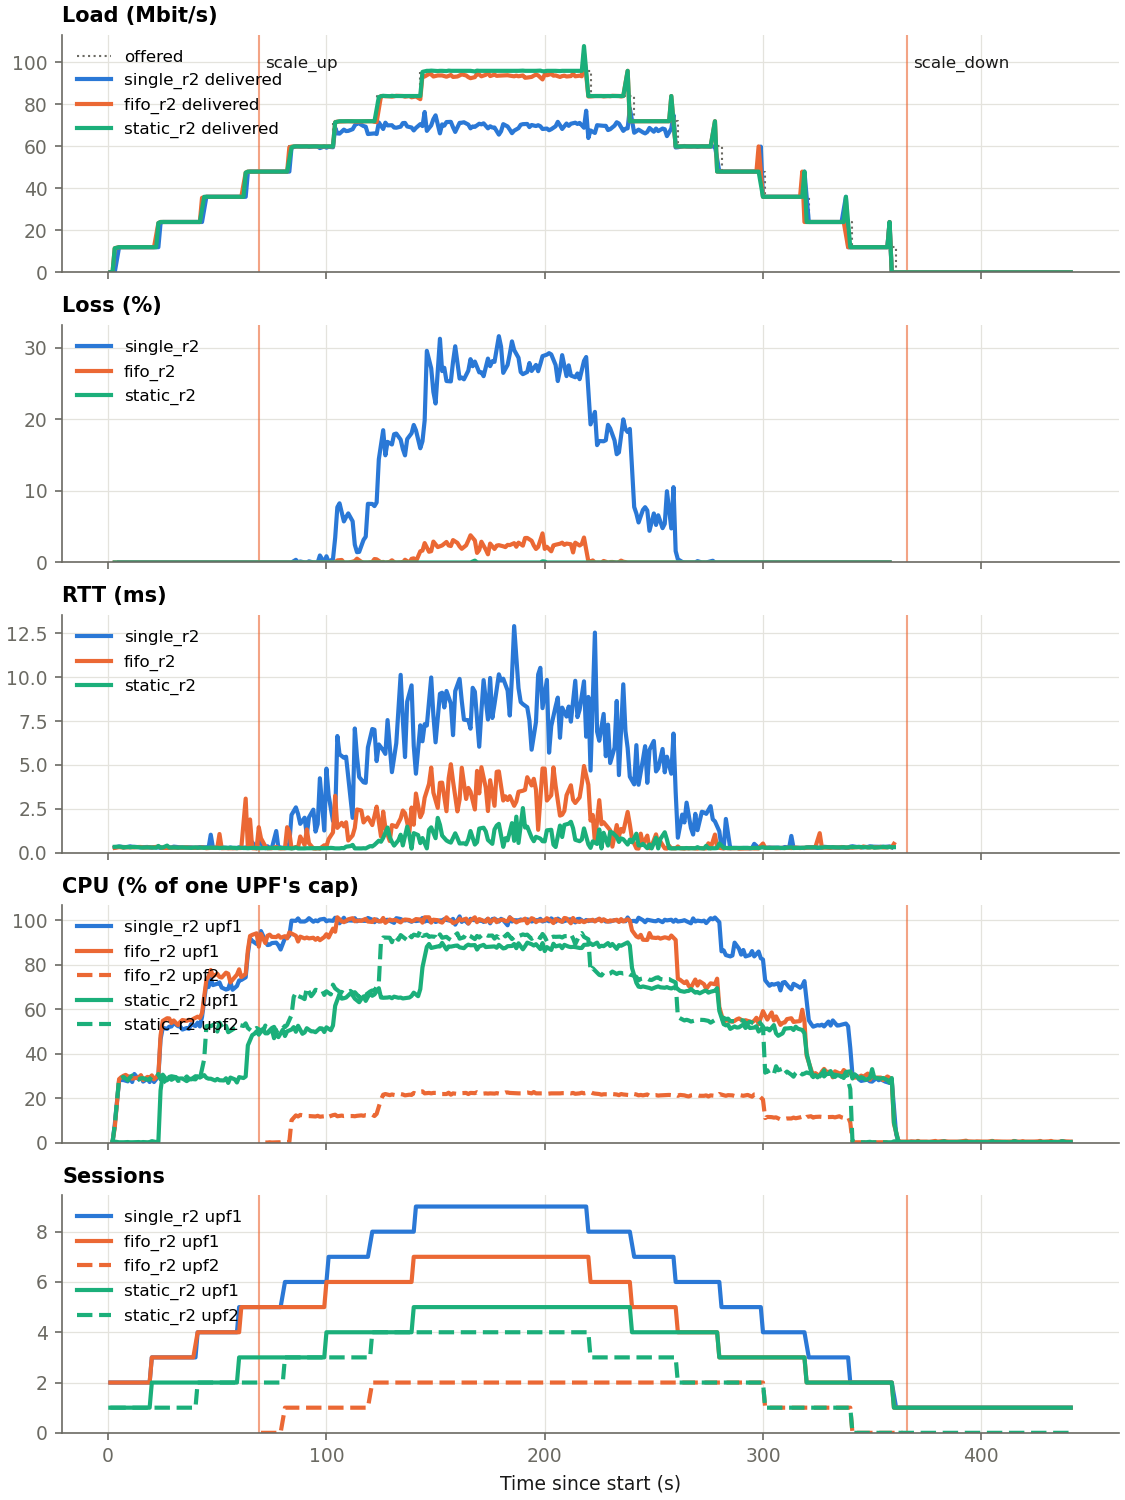
\includegraphics[width=\columnwidth]{single_r2_ramp.png}
\caption{Ramp with one UPF (repetition 2): delivered traffic stops growing at about 69~Mbit/s once the 6th UE joins.}
\label{fig:ramp}
\end{figure}

The controller fired at 69--70~s in all three runs, right after the 4th UE joined (48~Mbit/s, upf1 over 80\%), and upf2 was associated 5.4--6.5~s later (3.3--6.5~s over all 15 controller runs of Sections~\ref{sec:compare} and~\ref{sec:down}). The ranges of the three set-ups do not overlap. Loss falls from 27.9\% to 3.9\% and RTT from 8.7 to 3.7~ms.

The scaled set-up does not reach the 0.0\% of the static one, for two reasons that Section~\ref{sec:second} explains. First, the 4 UEs placed before the scale-up stay on upf1 to the end, because sessions never move. Second, new sessions keep alternating, so UEs~6 and~8 still go to the busy upf1, which ends up with 6 UEs (72~Mbit/s) against a capacity of about 68. UEs~5 and~7 on upf2 see 0.0\% loss. (Per-UE loss, for example 1.9\% on average for the UEs on upf1, is taken over each UE's whole run, including the time before saturation, so it is lower than the steady-state figure.)

\section{Removing the Second UPF}\label{sec:down}
After 60~s at full load, one UE stops traffic and deregisters cleanly (\texttt{deregister switch-off}) every 20~s. UEs~5 and~7 are on upf2 in every run. Five variants, 3 runs each (Table~\ref{tab:down}); ``fits on one'' means offered load below 45~Mbit/s.

\begin{table}[t]
\centering
\caption{Scale-down variants (means of 3 runs). upf2 idle: time upf2 ran with 0 sessions. Both UPFs after fit: time both ran after the load fitted on one. lifoearly is lifo with \texttt{--empty-down}; forced is upf2last with \texttt{--drain-timeout 30}.}
\label{tab:down}
\footnotesize
\setlength{\tabcolsep}{2.5pt}
\begin{tabular}{>{\raggedright\arraybackslash}p{1.2cm}>{\raggedright\arraybackslash}p{1.5cm}>{\raggedright\arraybackslash}p{1.1cm}>{\raggedright\arraybackslash}p{1.1cm}>{\raggedright\arraybackslash}p{1.1cm}>{\raggedright\arraybackslash}p{1.4cm}}
\toprule
Variant & UEs leave & upf2 stopped (s) & upf2 idle (s) & Both UPFs after fit (s) & Lost \\
\midrule
fifo & 1, 2, \dots, 8 & 365 & 25 & 64 & nothing \\
lifo & 8, 7, \dots, 1 & 366 & 86 & 65 & nothing \\
lifoearly & 8, 7, \dots, 1 & 326 & 45 & 25 & nothing \\
upf2last & upf2's UEs last & 451 & 0 & 150 & nothing \\
forced & upf2's UEs last & 381 & 0 & 80 & 10.7~s, new IP \\
\bottomrule
\end{tabular}
\end{table}

\begin{figure}[t]
\centering
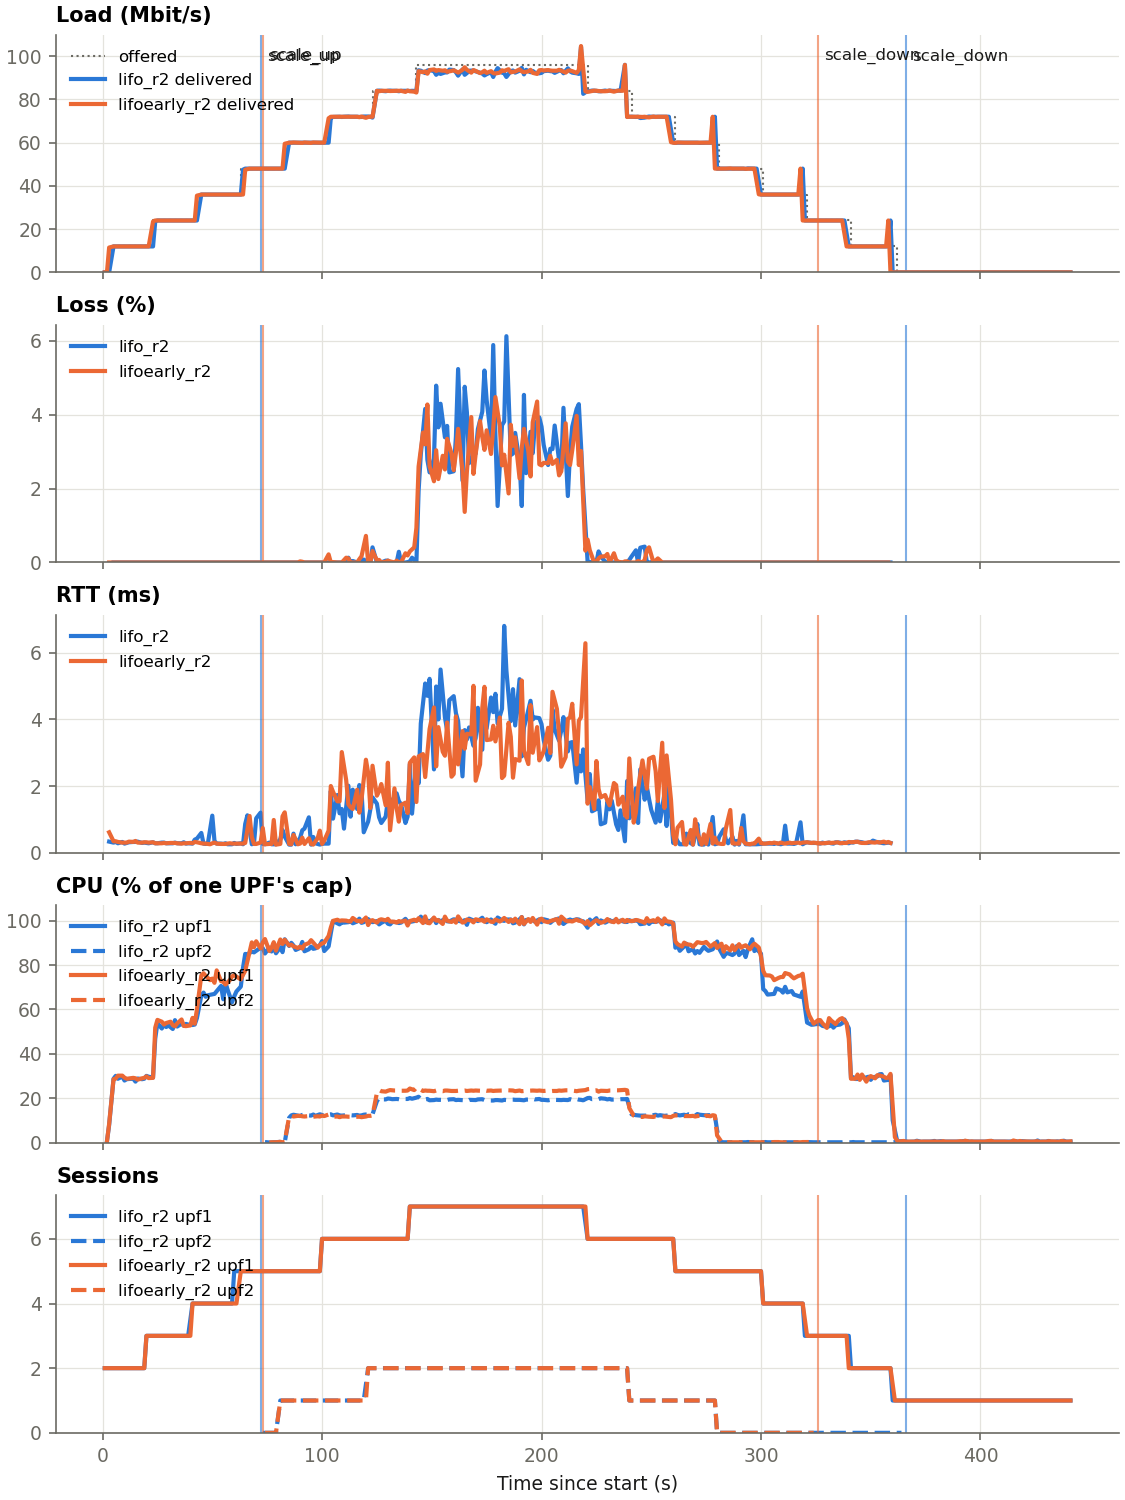
\includegraphics[width=\columnwidth]{lifo_r2_ramp.png}
\caption{Ramp-down (repetition 2): default rule vs.\ \texttt{--empty-down}.}
\label{fig:down}
\end{figure}

\begin{figure}[t]
\centering
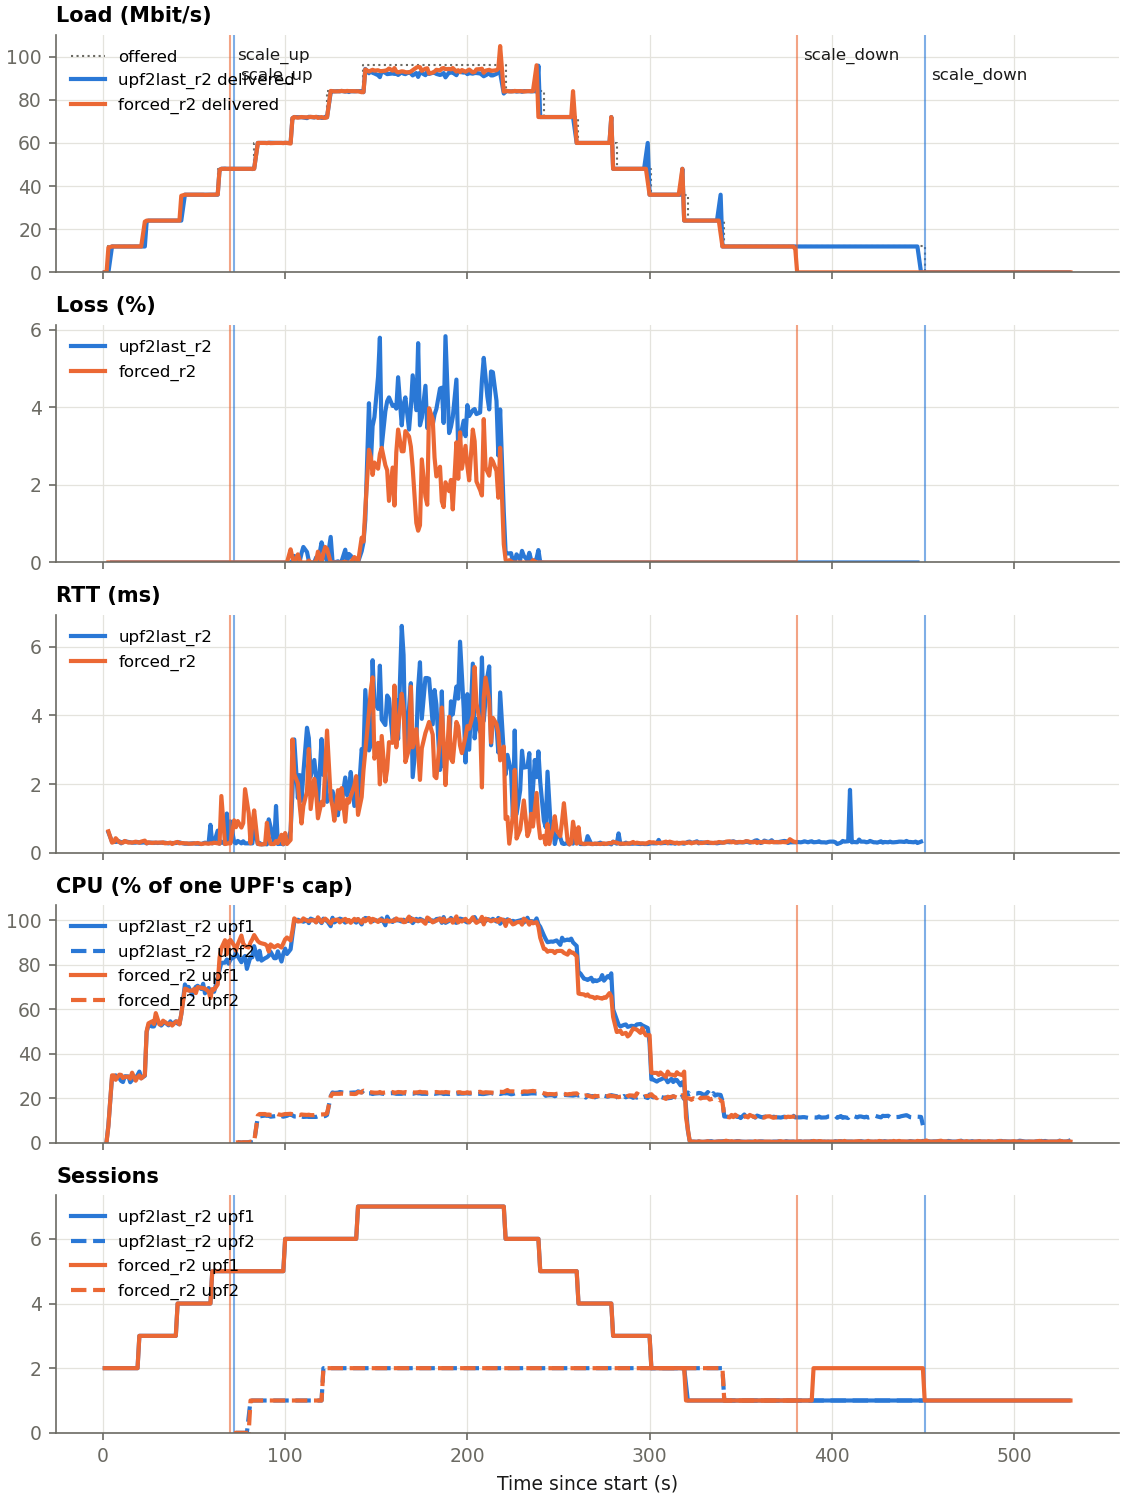
\includegraphics[width=\columnwidth]{upf2last_r2_ramp.png}
\caption{Ramp-down where upf2's UEs leave last (repetition 2): waiting for the last session (graceful) vs.\ \texttt{--drain-timeout} (forced).}
\label{fig:down2}
\end{figure}

\begin{itemize}
\item \textbf{Waiting for 0 sessions loses nothing} in all 12 runs that waited (mean loss at most 0.06\%), but it has no upper bound. In upf2last, one 12~Mbit/s UE kept upf2 running for 150~s after one UPF would have been enough, and would have kept it forever had it never left.
\item \textbf{An empty upf2 is waste.} In lifo, upf2 ran 86~s with no sessions. \texttt{--empty-down} stops it 40~s sooner at no cost, because an empty UPF carries no traffic, and it still waits while upf1 is busy.
\item \textbf{Forcing bounds the wait but costs traffic.} After stopping upf2 with a live session, the SMF noticed only through missed PFCP heartbeats and released the session. The UE re-established it on upf1 with a \emph{new IP address}: 10.7~s (10--12) without traffic in 3 of 3 runs. An application bound to the old address would have to reconnect.
\end{itemize}

\section{Limitations of Dynamic UPF Scaling in Open5GS}\label{sec:limits}
\begin{enumerate}
\item \textbf{Selection is round-robin, not load-aware.} The only selectors are static (DNN, TAC, cell ID). After scale-up, every other new UE still goes to the saturated UPF.
\item \textbf{Existing sessions never move.} Scaling relieves only future load.
\item \textbf{No graceful drain.} The SMF cannot be told to stop choosing a UPF. A UE that dies without deregistering left its session counted on upf2 for over 60~s, so upf2 is never retired.
\item \textbf{Scale-down is all-or-nothing per UPF.} The controller can only wait or cut; it cannot move the last UE to upf1 first.
\item \textbf{Scale-up is slow:} 5~s hold plus 3--7~s (up to the SMF's 11~s retry period) before upf2 is used.
\item \textbf{A shared UE pool needs NAT on N6.} The data network sees the UPF's address, not the UE's.
\item \textbf{Thresholds are host-dependent in Mbit/s}, so they must be re-derived per host and cap, and kept as a share of the cap.
\item \textbf{Per-second signals are noisy} (throttling swings by 10--15 points at steady load); smoothing and a hold time are required.
\end{enumerate}

\section{Threats to Validity}
The 0.1-core cap is artificial and capacity is in CPU-time units, not real UPF throughput. Traffic is uplink UDP from simulated UEs; there is one gNB, one slice and at most two UPFs. Each set-up has only three repetitions, though the ranges are far apart, and all results come from one host in one session. An earlier session on the same laptop, with a slower CPU setting, showed the same qualitative picture (1 UPF: 19.3\% loss, controller: 0.5\%, 2 UPFs: 0.0\% at 64~Mbit/s), but with different absolute numbers. The host must also be quiet: one repetition was discarded after other applications exhausted memory.

\section{Conclusion}
At a 0.1-core cap one UPF carries about 68~Mbit/s and degrades from about 60. A controller using only UPF CPU, with a threshold about three quarters of the way to the knee, can add a second UPF without restarting the core, cutting loss at 96~Mbit/s from 27.9\% to 3.9\%. The remaining loss comes from Open5GS itself: strict round-robin placement and sessions that never move. Removal is safe if the controller waits for the second UPF to empty, but the wait is unbounded, and forcing it costs the affected UE about 11~s and its IP address. A core that could place new sessions by load, or move or steer sessions away from a draining UPF, would remove both problems.

\textbf{Code and data.} Everything is in the project repository, submitted separately. Table~\ref{tab:thr} comes from \texttt{results/final/threshold.csv} (one row per run, with a validity flag, host load and power state); Tables~\ref{tab:cmp}--\ref{tab:down} from the per-second timelines and per-UE files in \texttt{results/final/ramp/} (\texttt{summary.md} holds the full tables, \texttt{host.txt} the host state); Table~\ref{tab:trace} from the N4 and N3 captures in \texttt{results/linux/trace\_r1..r3/} (\texttt{.pcap}, openable in Wireshark, with \texttt{sessions.csv}). \texttt{results/linux/} also holds the earlier calibration. The whole final session reruns with \texttt{final.sh}.

\begin{thebibliography}{1}
\bibitem{ts23501} 3GPP, ``System architecture for the 5G System (5GS),'' TS 23.501.
\bibitem{ts29244} 3GPP, ``Interface between the Control Plane and the User Plane nodes (PFCP),'' TS 29.244.
\bibitem{open5gs} Open5GS, \url{https://open5gs.org}.
\bibitem{ueransim} UERANSIM, \url{https://github.com/aligungr/UERANSIM}.
\end{thebibliography}

\end{document}
